% This document provides the style to be used for a MSc Thesis at the
% Parallel and Distributed Systems group
\documentclass[11pt,twoside,a4paper,openright]{report}

% math packages
\usepackage{amsthm}
\usepackage{amsmath}
\usepackage{amssymb}
\usepackage{subfig}
 \usepackage{floatrow}
\usepackage{algorithmicx}
\usepackage{algorithm}
\usepackage{algpseudocode}

% textblocks for title page
\usepackage[absolute]{textpos}
\usepackage{tikz}

% use babel for proper hyphenation
\usepackage[british]{babel}
\usepackage[numbers]{natbib}
\usepackage{bytefield}

% Graphics: different for pdflatex or dvi output, choose one
%%\usepackage[dvips]{graphicx}
%%\usepackage[pdftex]{graphicx}
\usepackage{graphicx}

\usepackage{epstopdf}
\usepackage{rotating}


% FONT
\usepackage[scaled=.92]{helvet}
%\usepackage{times}

% for url's use "\url{http://www.google.com/}"
\usepackage{url}
\usepackage{hyperref}

\hypersetup{
  colorlinks   = true, %Colours links instead of ugly boxes
  urlcolor     = cyan, %Colour for external hyperlinks
  linkcolor    = cyan, %Colour of internal links
  citecolor   = cyan %Colour of citations
}
\usetikzlibrary{shapes,arrows,graphs,positioning,automata,shadows,fit,shapes,decorations.pathreplacing}
\tikzset{
    rotate around with nodes/.style args={#1:#2}{
        rotate around={#1:#2},
        set node rotation={#1},
    },
    rotate with/.style={rotate=\qrrNodeRotation},
    set node rotation/.store in=\qrrNodeRotation,
}

\def\algbackskip{\hskip\dimexpr-\algorithmicindent+\labelsep}
\def\LState{\State \algbackskip}%
% Information that will be filled in at various points in the report
\newcommand{\reportTitle}{TODO TITLE}
\newcommand{\reportAuthor}{Arpan Govindraju}
\newcommand{\reportEmail}{a.govindaraju@student.tudelft.nl}
\newcommand{\reportUrlEmail}{\href{mailto:\reportEmail}{\reportEmail}}
\newcommand{\reportMSC}{MSc Embedded Systems} %{Embedded Systems}{Computer Engineering}{Computer Science}{Electrical Engineering}
\newcommand{\reportDate}{\today} %TODO: Dit is de datum van uitgifte van final versie aan de afstudeer commissie 
\newcommand{\presentationDate}{\today} %TODO: Dit is de datum van de afstudeerpresentatie 
\newcommand{\graduationCommittee}{
TODO GRADUATION COMMITTEE & Delft University of Technology \\
TODO GRADUATION COMMITTEE & Delft University of Technology \\
} % The order of listing the names: Graduation prof, supervisor(s), others ordered by title + alphabetical 
%examples: 
%prof. dr. ir. H. J. Sips (chair) & Delft University of Technology \\ 
%ir. dr. D. H. J. Epema           & Delft University of Technology \\ 
\newcommand{\reportAbstract}{TODO ABSTRACT}
\newcommand{\reportKeywords}{TODO KEYWORDS}
%\newtheorem{theorem}{Theorem}[section]
\theoremstyle{definition}
\newtheorem{definition}{Definition}[section]


% For pdflatex
\pdfinfo{
   /Author (\reportAuthor)
   /Title  (\reportTitle)
   /Keywords (\reportKeywords)
}

\begin{document}

\pagenumbering{alph}
\pagestyle{empty}


% FRONTCOVER
%%\usepackage[total={210mm,297mm},left=0pt,bottom=0pt,top=0cm,right=0pt,headsep=0pt,head=0pt,showframe]{geometry}

%%\input{preambleL31958}
%%\begin{titlepage}
\begin {textblock*}{210mm}(0mm,0mm)
\noindent

\includegraphics[height=3.2cm]{pics/block}
\sffamily
\vspace{.8cm}
\begin{center}
\Large
Delft University of Technology\\
Master's Thesis in \reportMSC\\
\vspace{2cm}
\parbox{170mm}{\bfseries\centering\Huge\reportTitle}\\
\vspace{1cm}
\parbox{170mm}{\bfseries\centering\reportAuthor}

\end{center}
\end{textblock*}

\begin {textblock*}{210mm}[0.0,1.0](0mm,297mm)
\noindent
\hspace{1.5cm}
\hfill\parbox{5cm}{

\includegraphics[scale=1]{pics/philips_lighting.png}}
\hspace*{2cm}\\

\vspace*{1cm}

\hfill\parbox{5cm}{

\includegraphics[width=5cm]{pics/es_logo_cyan_black_rgb}}
\hspace*{2cm}\\

\vspace*{1.5cm}
\noindent

\includegraphics[width=\textwidth]{pics/TU_border_A4_L_front}
\end{textblock*}

\null\newpage


%%%%%%%%%%%%%%%%%%%%%%%%%%%%%%%%%%%%%%%%%%%%%%%%%%%%%%%%%%%%%%%%%%%%%%%%%%%%%%%
\hoffset=1.63cm
\oddsidemargin=0in
\evensidemargin=0in
\textwidth=5in

%%%%%%%%%%%%%%%%%%%%%%%%%%%%%%%%%%%%%%%%%%%%%%%%%%%%%%%%%%%%%%%%%%%%%%%%%%%%%%%
\parindent=1em

% EMPTY PAGE
\cleardoublepage

\pagestyle{plain}
\pagenumbering{roman}
\setcounter{page}{1}

% TITLE PAGE: page i (hidden)
\begin{titlepage}

  \begin{center}
  \null\vfill
    \begin{center}
    \LARGE{\reportTitle}
    \end{center}

    \vspace{3cm}

    \begin{large}
    Master's Thesis in \reportMSC
    \end{large}

    \vspace{1.5cm}

    \begin{normalsize}
    Embedded Software Section\\
    Faculty of Electrical Engineering, Mathematics and Computer Science\\
    Delft University of Technology\\
    Mekelweg 4, 2628 CD Delft, The Netherlands
    \end{normalsize}

    \vspace{2.0cm}

    \begin{normalsize}
    \reportAuthor \\
    \reportUrlEmail
    \end{normalsize}

    \vspace{1.0cm}

    % <MM> DD, YYYY
    \reportDate             %TODO: Dit is de datum van uitgifte van final versie aan de afstudeer commissie

  \vfill
  \end{center}

\end{titlepage}


% GRADUATION DATA AND ABSTRACT: pages ii and iii (hidden)
%De aankondiging bevat de spreker, titel, plaats, datum en tijd, samenstelling van de afstudeercommissie en een korte samenvatting (maximaal 25 regels).
\thispagestyle{empty}

\noindent \textbf{Author}\\
\begin{tabular}{l}
\reportAuthor{} (\reportUrlEmail)\\
\end{tabular}\\
\noindent \textbf{Title}\\
\begin{tabular}{l}
\reportTitle\\
\end{tabular}\\
\noindent \textbf{MSc presentation}\\
\begin{tabular}{l}
% <MM> DD, YYYY (like \today)
\presentationDate\\
\end{tabular}

\vspace{1.1cm}

\noindent \textbf{Graduation Committee}\\
\begin{tabular}{ll}
\graduationCommittee
\end{tabular}


\begin{abstract} %de abstract bevat alleen een korte samenvatting van de inhoud van het onderzoek
\setcounter{page}{3}
\reportAbstract{}
\end{abstract}

\clearpage

%\setcounter{page}{4}

% EMPTY PAGE: page iv
\cleardoublepage

% OPTIONAL QUOTATION: page v
%\pagestyle{empty}

\null\vfill

\begin{center}
\emph{`Location, Location, Location''} -- Harold Samuel
\end{center}

\vspace{10cm}

\clearpage


% EMPTY PAGE: page vi
%\cleardoublepage

% PREFACE: page v
\chapter*{Preface}
\addcontentsline{toc}{chapter}{Preface}


\vspace{1\baselineskip}

\noindent
Indoor spaces are getting smarter day by day with deployment of huge amount of sensors and actuators. Many applications built for maintenance of the building use the sensor data as inputs to actuate the actuators to perform their function. May it be simple turning on and off of lights based on occupancy or a more critical applications like fire detection and alarming, all need data from the sensors. One important meta-data about the sensor, that is crucial for all theses application is the sensor location. Without which the applications cannot perform effectively. Till now the meta-data is being created and maintained manually, which is a cumbersome process and prone to error. In our work here we propose a method to automatically determine the location of the sensor using the data from the sensors.

This work was carried out at Philips Lighting, Eindhoven. Philips Lighting being a market leader in the field of lighting are actively providing lighting control solutions. This work is aimed to help automate the process of creating and maintaining the meta-data of sensor location and thus aiding faster deployment and easier maintenance of the systems.

Before going to the technical details of the thesis, I would like to thank my supervisor Dr.Ashish Pandharipande(Philips Research) for giving me an opportunity to carry out my thesis at Philips Lighting. I would also like to thank him and Dr.David Caicedo Fernandez(Philips Research) for critically analyzing my work during our regular weekly meetings and giving me valuable suggestions. My sincere gratitude to my university supervisor Dr.Venkatesh Prasad(TU Delft) for all the support and guidance he provided. I would also like to thank my parents and grandparents for all their unconditional love and support during all these years.
I would like to thank all my friends who have tolerated my constant whining and supported me during my tough times.
A special thanks to all the people of FO 52 and interns room past and the present who made the stay in Eindhoven so much more pleasant.

\vspace{1\baselineskip}

\noindent
Arpan Goindaraju\\
%\vspace{1\baselineskip}
%\noindent
Eindhoven, The Netherlands\\
%\noindent
\today

% EMPTY PAGE: page vi
\cleardoublepage

% TABLE OF CONTENTS: starting at page vii
\tableofcontents

\cleardoublepage

\pagenumbering{arabic}
\setcounter{page}{1}

% INTRODUCTION: page 1
\chapter{Introduction}
\label{chp:introduction}
\section{Motivation}
The European Union (EU) has pledged to cut the consumption of primary energy by 20\%, by the year 2020.  It is estimated that buildings consume 40\% of the energy produced\footnote{according to value published at https://ec.europa.eu/energy/en/topics/energy-efficiency/buildings }.  This has resulted in an increase in the demand to reduce the energy consumption of buildings. To reduce the consumption of energy, building automation systems (BAS) are being widely employed. BAS are computer-based systems that help to manage, control and monitor building technical services (HVAC, lighting etc.) and the energy consumption of devices used by the building. It is estimated that BAS can save a building between 5 percent to 30 percent on the utility cost by managing HVAC and lighting systems\cite{bas}.

BAS deploy a huge amount of sensors, which provide inputs to perform efficient control of various services. BAS brings with it various benefits, at the same time, offers numerous challenges too. For BAS, sensor measurements alone are not sufficient to understand the condition of the facilities, unless combined with meta-data associated with the sensors.
Meta-data as defined in \cite{gao2015data} refers to any information associated  with the device that help to contextualize the measurements or control signals regularly being sent from/to the device, such as the location within the building, the physical phenomenon being sensed, etc. One of the major challenges in a BAS system is generating and updating the meta-data of the sensor.
One of the important meta-data required is that of the physical location of the sensor as discussed in  \cite{liu2009requirements}.
As the size and distribution of the deployed sensors are high, it is highly cumbersome and error prone to manually maintain the meta-data about the sensor placement. Apart from being error prone, the manual configuration has to be repeated every time there is a change in the meta-data. Change in meta-data can be due to various reasons, such as a change in the office setup, replacement and/or relocation of sensors. All these factors result in inaccurate information about the location of the sensors. Without the accurate information of the location of the sensors, interpreting the data collected from the sensor is difficult and also can be misleading. This could result in the decrease in the effectiveness of the deployed BAS systems. Hence there is a need to develop methods to accurately determine the location of the sensors within the building.
\section{System Description}
Smart lighting control is one of the major component of BAS. Lighting is responsible for 11 percent  and 18 percent of the energy consumption in case of residential and commercial buildings respectively\cite{website}. 
State of the art lighting control employs co-located occupancy sensors and light sensors, placed on luminaries which are attached to the ceiling\cite{pandharipande2015smart,caicedo2016smart,van2014distributed}.
In this thesis, we consider such ceiling based sensor grid consisting of occupancy sensors. We represent the sensor grid as a graph $G$ with the sensors located on the vertices of the graph.

\section{Problem Statement}

Several studies \cite{Hong:2013:TAS:2528282.2528302,doi:10.1061/9780784413616.226,Koc:2014:CLC:2674061.2674075,Lu:2014:SBS:2648771.2629441,ellis2012creating,muller2014automated,marinakis2005learning} have been carried out to infer the sensor location from sensor data. Most of the methods developed so far have identified ways to cluster the sensors that are located within their proximity; however the methods do not identify where exactly on the grid each sensors are located in a dense sensor grid \cite{Hong:2013:TAS:2528282.2528302,doi:10.1061/9780784413616.226,Koc:2014:CLC:2674061.2674075}.  Therefore the research question that is being tackled in this work is:

\textit{How to Automatically determine the location of the sensors utilizing binary data from the ceiling mounted occupancy sensors and the information about the grid (coordinates of the vertices constituting the grid)?}

\section{Contribution of the thesis}
The main contribution of the thesis are:
\begin{itemize}
\item Energy feature of the binary occupancy sensor data is used to distinguish between neighboring and non neighboring nodes.
\item Reducing the problem of determination of sensor locations  on the grid to a problem of graph matching \cite{conte2004thirty}.
\end{itemize}

\section{Outline of thesis}

The rest of the thesis is organized as follows: in chapter 2 we give a brief overview of related work. In chapter 3 we present the method that has been developed. In chapter 4 we describe our testbed setup. Next, in chapter 5 we present the results obtained by applying the method that we have developed on actual sensor data obtained from 2 different testbeds. In the end in chapter 6 we conclude the work done and discuss future work.


%\section{Application}
%FOr few of the applications like the one developed in 




\vspace{1\baselineskip}

\noindent
%TODO ORGANISATIONAL DESCRIPTION OF THESIS





% CHAPTERS ... For instance: History/Prior Work, Design/Implementation, Experiments
\chapter{Literature Review}
%In \cite{wang2010survey}  \citeauthor{wang2010survey} classify the problem of sensor localization into three categories: proximity based localization , range based localization and angle based localization.\\
%In \textbf{proximity based localization} few nodes are aware of there locations called the anchor nodes and the other nodes calculate their position relative to these anchor nodes.\\
%\textbf{Range based localization:} This localization is  based on the ranging techniques using RSSI, Time of Arrival, Time Difference of Arrival . Although computation of the distances between each pair of location is trivial, the problem of finding the locations given the pairwise Euclidean distance is not. Range based approach may %or may not need anchor nodes. With anchor based approach Multilateration technique is used to find the location of the non anchor nodes. Without anchor nodes multi dimensional scaling (MDS) is adopted for localization. \\
%\textbf{Angle based localization:} In Angle based localization method additional information of angle of arrival of the signal is used for the process of localization. To caclulate the angle of arrival antenna array or multiople receivers on the nodes are required.\\ 
%Though the above discussed methods are known to give good results in localizing the sensor networks. Theses methods are not likely to be applied in a large indoor environment like commercial office spaces . As these methods either need specialized hardware in the case of angle based localization or they need higher processing %power. Which result in the increase of the cost per sensor node.This gives rise for a need of an alternate solution. The other method of localizing the sensors within a facility is sensor data driven.\\ 
%This section provides an insight about the work that has been done in automatic identification of the sensor locations within a building using sensor data. Previous efforts on creating a data-driven sensor localization methods have identified ways to cluster the sensors that are located within the same room.However the existing %methods do not identify the locations of the sensors within the building. Previous work of \citeauthor{Hong:2013:TAS:2528282.2528302} and \citeauthor{fontugne2012empirical} \cite{fontugne2012empirical} have shown methods of clustering different sensors that fall within a room.\\ 
%In particular \citeauthor{Hong:2013:TAS:2528282.2528302}\cite{Hong:2013:TAS:2528282.2528302} extended the work done in \cite{fontugne2012empirical} and showed the existence of a statistical boundary between sensors analogous to the physical one exists and is empirically discoverable.
%In \cite{doi:10.1061/9780784413616.226} \citeauthor{doi:10.1061/9780784413616.226} propose a feature, energy content in HVAC delivered air, which can be derived from HVAC system sensors which could lead to identification of the space in which the sensors are located . \citeauthor{Lu:2014:SBS:2648771.2629441}%%%\cite{Lu:2014:SBS:2648771.2629441} and \citeauthor{ellis2012creating}\cite{ellis2012creating} describe methods to obtain floor map for the smart home from the sensor data. They are able to map the sensors to the room and obtain connectivity map between the rooms in the smart home.\\
%All the previous work look at identifying the sensors that are present in same room but they do not answer the question of which sensor is located where within the given space. In our work we propose a method to determine the position of the sensors within an indoor space given the possible locations of the sensors.

There has been an extensive body of research that aims at obtaining the location information of the sensors in WSN's. All the approach that has been taken till now has been categorized by \citeauthor{wang2010survey} in \cite{wang2010survey} to fall into one of the following categories:
\begin{itemize}
\item Proximity based localization
\item Range based localization
\item Angle based localization
\end{itemize}

In proximity based localization, WSN is represented as a graph $G(V,E)$. Location of the  subset of the nodes, $H \subset G$ are known. The goal is to estimate the location of the remaining $V-H$ nodes relative to the position of the $H$ nodes. 
Range based localization makes use of  ranging techniques using RSSI, time of arrival and time difference of arrival of the signals. The distance is computed using the ranging technique. Computing the locations of the nodes using distance information is non trivial. Range based approach may or may not need anchor nodes. With anchor based approach Multilateration technique is used to find the location of the non anchor nodes. Without anchor nodes, multi dimensional scaling (MDS) is adopted for localization. 
Angle based  localization uses the information of angle of arrival of the signals to determine the location of the sensors. To determine the angle, antenna array or multiple receivers on the node are required.

Apart from the techniques mentioned above, recently there have been few works which look at the data measured by the sensors to obtain the information about the location of the sensor. As our approach towards determining the sensor location uses sensor data as input, in this chapter we provide a brief overview of the works which take the same approach. 

Various approaches have been taken to automate the process of determining the sensors location using the data from the sensors in buildings using different data analytics and signal processing tools. \citeauthor{Hong:2013:TAS:2528282.2528302}\cite{Hong:2013:TAS:2528282.2528302}
 apply empirical mode decomposition to 15 sensors in 5 rooms to cluster sensors which belong to the same room by analyzing the correlation coefficients of the intrinsic mode functions. They characterize the correlation coefficient distribution of sensors that are located in the
 same room and different rooms. They were able to show that there exists a correlation boundary analogous to the physical boundary which can be discovered empirically. 
In \cite{doi:10.1061/9780784413616.226} \citeauthor{doi:10.1061/9780784413616.226} propose a feature: energy content in HVAC delivered air, which can be derived from HVAC system sensors which could lead to the identification of the space in which the sensors are located . They combine sensor measurements and building characteristics(floor area) for the identification of the space in which the sensors are present.
In \cite{Koc:2014:CLC:2674061.2674075} \citeauthor{Koc:2014:CLC:2674061.2674075} propose a method to automatically identify the zone temperature and discharge temperature sensors that are closest to each other by using a statistical method on the collected raw data. They explore whether linear correlation or a statistical dependency measure(distance correlation) are better suited to infer spatial relationship between the sensors. They carry out their analysis on three different testbeds. They also investigate the effects of distance between sensors and measurement periods on the matching results. In the end, the authors conclude that linear correlation coefficient provides better matching results compared to distance correlation. The authors also conclude that as the distance between the sensors increase, the data size needed to infer spatial relationships also increase.

\citeauthor{Lu:2014:SBS:2648771.2629441}\cite{Lu:2014:SBS:2648771.2629441} describe a method to generate representative floor plans for a house. Their method clusters sensors to a room and assigns connectivity based on the simultaneous firing of the sensors placed on the door and window jambs. The algorithm gives a small set of possible maps from which the user has to choose the right map. Method requires special placement of the sensors . The authors were able to calculate the floor map of 3 out of the 4 houses they evaluated.  
 \citeauthor{ellis2012creating}\cite{ellis2012creating} proposed an algorithm to compute the room connectivity using  PIR and light sensor data. They compute room connectivity based on the artificial light spill over between rooms; occupancy detection due to movements between
  rooms; and fusion of the two. They calculate the transition matrix for the light sensor and occupancy sensor. Fuse both the data together to compute the connectivity graph. Here the authors have considered a situation where there is only one PIR and light sensor per room.
\citeauthor{muller2014automated} define  sensor topology as a graph with directed and weighted edges. All pairs of consecutive sensors triggers are interpreted as a user walking from the former to the latter sensing region indicated in the sensor 
graph by an edge from the former to the latter. Every time a consecutive edge triggers are observed the weight of the edge between the sensors is incremented. They define a method to filter out erroneous edges.
In \cite{marinakis2005learning} \citeauthor{marinakis2005learning} obtain the sensor network topology using Monte Carlo Expectation Maximization. They assign activity to people present in the space to obtain the graph topology. The algorithm requires, number of people present in the space as the input. They demonstrate the effectiveness of the algorithm using various simulated data. 




%\section{Subgraph Isomorphism}
%
%In our work we reduce the problem of mapping the sensors to its location in the grid to graph matching problem. A graph matching process between two graphs $G$ = $(V_G,E_G)$ and H = $(V_H,E_H)$ consists of determining a mapping M which associates nodes of the graph G to H and vice versa. Different constraints can be imposed onto M which results in different mapping types: monomorphism, isomorphism, graph-subgraph isomorphism are the most popular ones.Graph matching is widely used in pattern recognition for comparing the graph representing an object to a model  graph, or prototype. Our problem falls under the category of graph monomorphism .  
%Most of the algorithms for graph matching are based on some form of tree search with backtracking. The basic idea is that the partial mapping (initially empty) is iteratively expanded by adding to it new pairs of matched nodes; the pairs are chosen based on some conditions employed to satisfy the conditions of the matching type.
%The first significant and most widely used algorithm in the area of graph matching was proposed by \citeauthor{Ullmann:1976:ASI:321921.321925} \cite{Ullmann:1976:ASI:321921.321925}. Ullmann algorithm addresses the problem of graph isomorphism, sub graph isomorphism , graph monomorphism. To prune unfruitful matches the author proposes a refinement procedure, which employ conditions based on the knowledge of the adjacent nodes and the degree of the nodes that are being matched. 
%\citeauthor{4308468} in \cite{4308468} propose a graph monomorphism algorithm. The major drawback of the algorithm is that the algorithm uses a $N^2 \times N^2$ matrix to represent netgraph
%. N represent the number of nodes of the largest graph. As a result of this only small graphs can be dealt with using the algorithm.  
%A more recent algorithm for graph isomorphism, subgraph isomorphism and monomorphism was proposed by \citeauthor{906251} in \cite{906251}, popular as VF algorithm. The authors define a heuristic that is based on the analysis of sets of nodes adjacent to the ones already considered in the partial mapping. The authors further improved the algorithm in 2001 in there paper \cite{cordella2001improved}. 
%The authors proposed a modification to the algorithm(called VF2) which reduces the memory consumption from $O(N^2)$ to O(N) where N is the number of nodes in the graph, thus enabling the algorithm to work with large graphs.
%In our work we use the VF2 algorithm to obtain the mappings between the spanning tree and grid graph.

% CONCLUSIONS AND FUTURE WORK
\chapter{Methodology}

\section{Data Description}
As it has been shown in \cite{Hong:2013:TAS:2528282.2528302} correlation values 
Data obtained from the PIR sensros is binary in nature. 1 indicates occupancy and 0 indicates non occupancy. \\
First step to determine the sensor location is to cluster the neighboring sensors together. Since neighboring sensors observe the same event, correlation value between the neighboring sensors should be high. So we compute the correlation coefficient of the raw data. To calculate the correlation between the binary data we use  the formula 
\begin{equation}
correlation ratio = \frac{a^2}{p_1\times p_2}
\end{equation}
a : number of 1’s in the same position in both the data.\\
P1: number of 1’s in data set 1.\\
P2:number of 1’s in dataset 2.\\

\section{Feature Extraction}
Energy feature is computed on 36 sample windows of pir sensor data with 18 samples overlapping between consecutive windows. At sampling frequency of 100ms, window length of 36 corresponds to 3.6s data.
The energy of bianry signal x(n) is computed as given in \ref{eq:energyEq}.\\
\begin{equation}
\label{eq:energyEq}
E_s = {\sum_{n=-\infty}^{\infty}{|x(n)|}^2}
\end{equation}
Energy of PIR signal along with giving the indication that the region is occupied it also gives information about the extent of activity in the region of occupancy. To diffrentiate between the neighboring nodes and non neighboring nodes we use pearson correlation coefficient given by \ref{eq:corrcoeff}. 
\begin{equation}
\label{eq:corrcoeff}
r(x,y)=\frac{\sum_{i=1}^{n}(X_i-\overline{X})(Y_i-\overline{Y})}{\sqrt{\sum_{i=1}^{n}(X_i-\overline{X})^2}\sqrt{\sum_{i=1}^{n}(Y_i-\overline{Y})^2}} \\
\end{equation}
X and Y are sensor data stream for sensor X and Y.\\
\overline{X} and \overline{Y} is the mean value of X and Y respectively.\\
n is the number of samples in sensor data stream.\\


 



\chapter{Test Bed}
\label{chp:testbed}
We setup our testbed in an $8m\times6m$ office space. Sensors are mounted on the ceiling which is at a height of 3m. The sensors are  placed 2.5m apart in the horizontal direction and 2.2m apart in the vertical direction. A schematic representation of the lab is as shown in the Figure \ref{fig:roomLayout} with the positions of the sensors marked. We use  PIR sensor, EKMB1101112 from Panasonic. 
The output of the sensor is binary, with 1 indicating occupancy and 0 if the region is unoccupied.  We use the sensors with eZ430-RF2500 toolkit which consists of MSP430 micro-controller  and CC2500 multi-channel
RF transceiver for wireless communication. The testbed uses simpliciTI a TI proprietary  low-power RF network protocol.  We mount all the 8 sensors on the ceiling of the room as shown in the Figure \ref{fig:photo}. 
All the 8 nodes communicate directly to a centrally located access point which is connected to a laptop, which stores the data.

\begin{figure}[!ht]
\centering
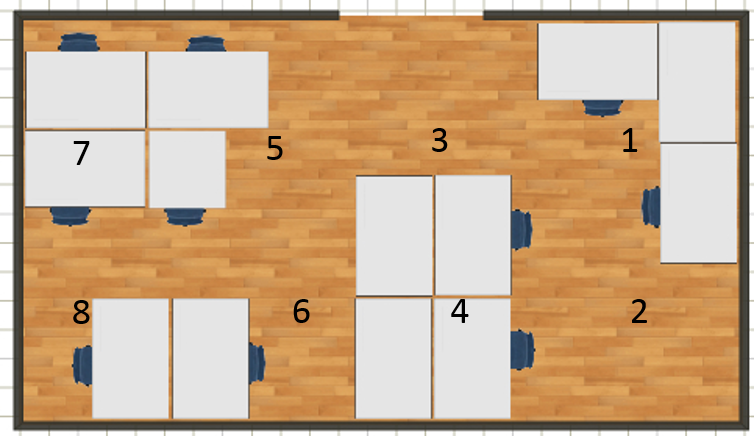
\includegraphics[scale=0.5]{./pics/roomLayout.png}
\caption{Room layout of the testbed.}
\label{fig:roomLayout}
\end{figure}


\begin{figure}[!ht]
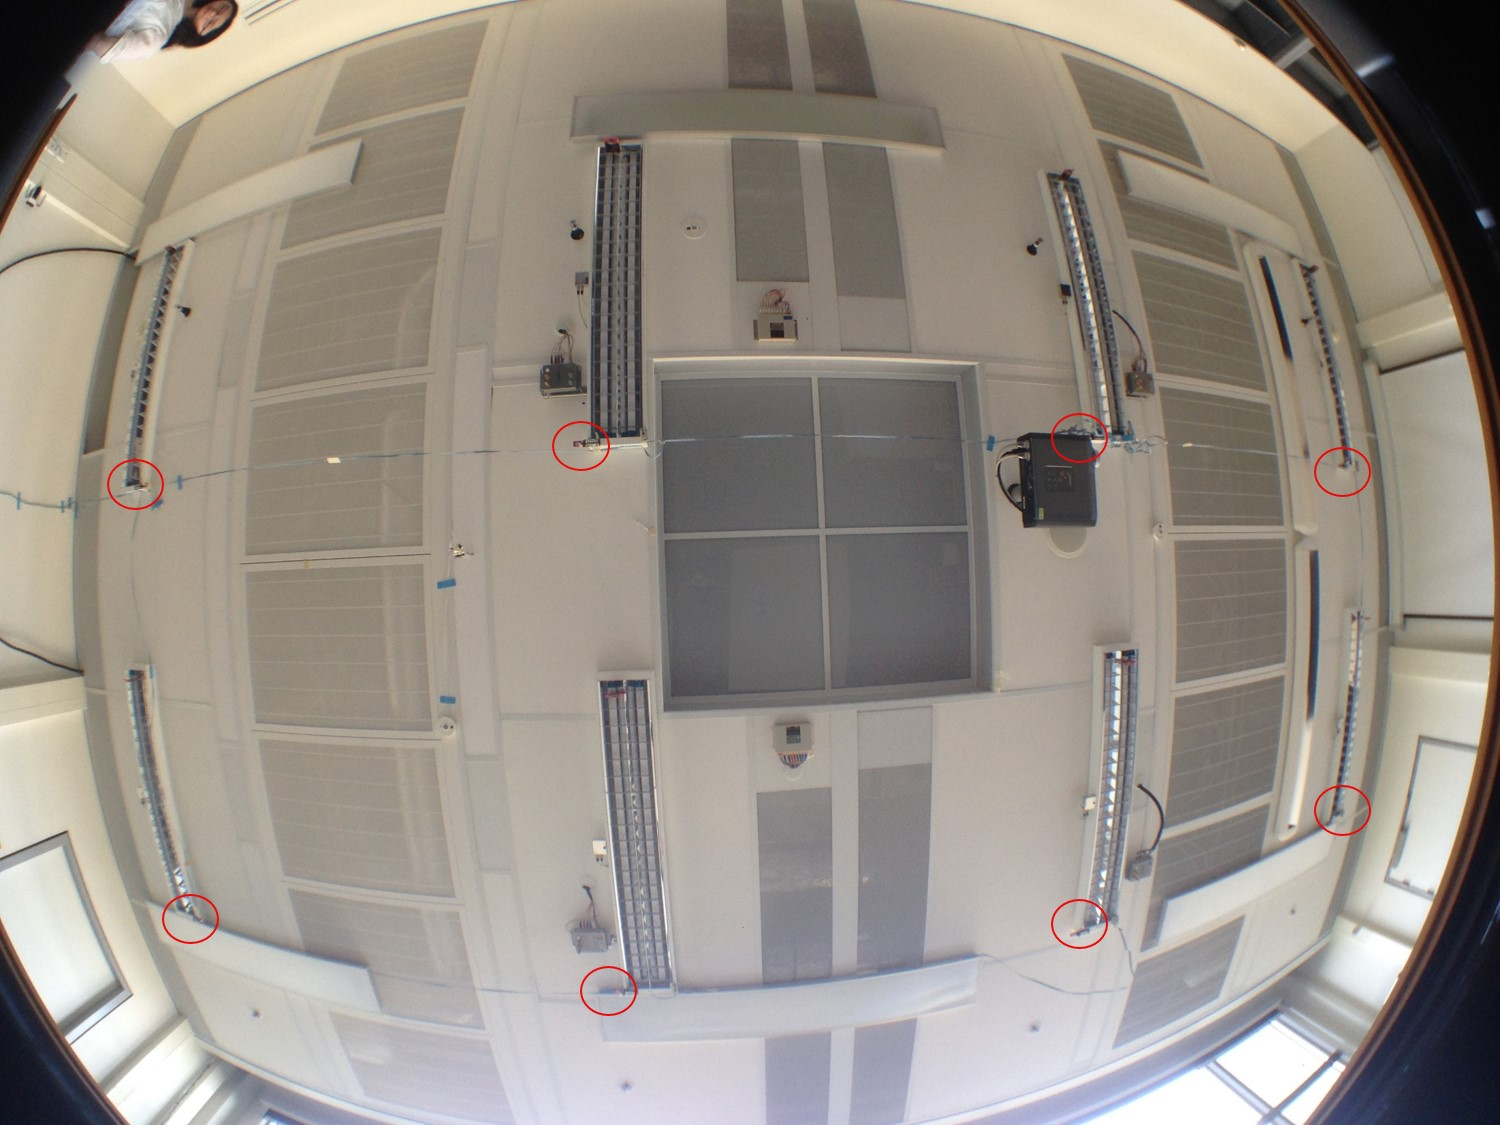
\includegraphics[scale=0.5]{./pics/lab_photo.jpg}
\caption{Photo of the lab setup with the sensors highlighted in red}
\label{fig:photo}
\end{figure}

\section{Packet Loss}
To avoid collision between the transmitted packets CSMA/CA is employed in our testbed. Even though CSMA/CA is employed, during our initial tests we observed packet loss as high as 23\% for few nodes as shown in the Figure \ref{fig:ackDis} and Table \ref{tab:packetLoss}. To decrease the packet loss we enable acknowledgment. An acknowledgment (ack) is sent from the AP if the packets are received. If no ack is received by a node, the node retransmits its data a maximum of 5 times until an ack is  received from the AP. If no ack is received even after 5 retransmission the packet is dropped and the next packet is prepared for transmission. From the Figure \ref{fig:ackEnb} and Table \ref{tab:packetLoss} we can see that the there was a decrease in the packet loss per node after ack was enabled. 

\begin{figure}[!ht]
    \centering
    \begin{subfigure}[b]{1\textwidth}
        \centering
        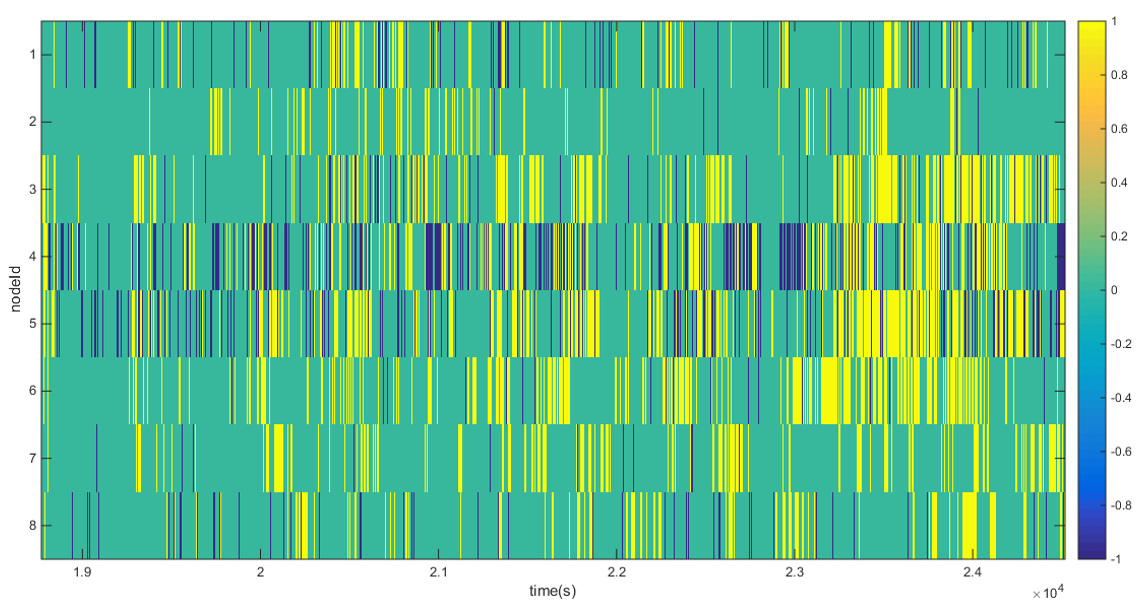
\includegraphics[width=8cm,height=4cm]{./pics/packetLoss.png}
      \caption{Data before ack was enabled}
       \label{fig:ackDis}
    \end{subfigure}
    \hfill
    \begin{subfigure}[b]{1\textwidth}
        \centering
        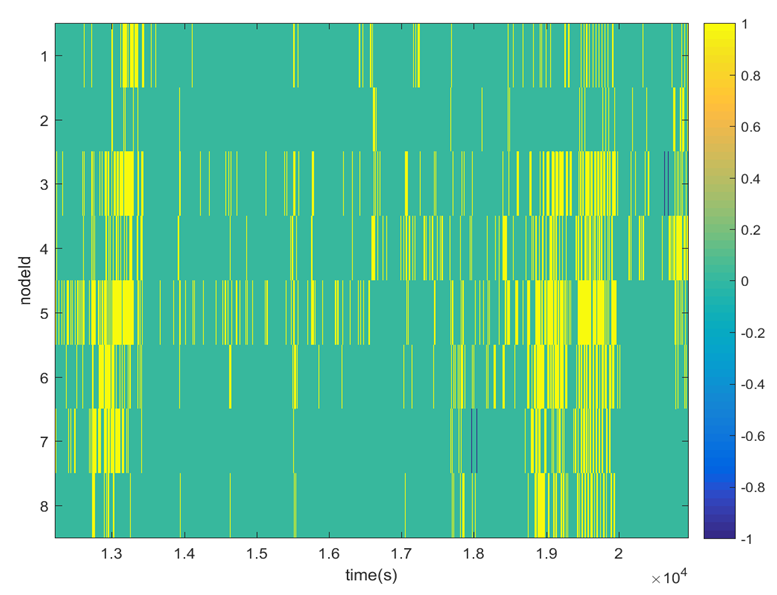
\includegraphics[width=8.5cm,height=4cm]{./pics/dataAfterAck.png}
        \caption{Data after ack was enabled}
        \label{fig:ackEnb}
    \end{subfigure}
\caption{Data from the test bed. - 1 indicates the lost data , 1 indicates occupancy, 0 indicates unoccupied space}
\label{fig:packetLoss}
\end{figure}

\begin{table}[!ht]
\centering
\caption{Packet loss without and with ack for all the sensor nodes}
\label{tab:packetLoss}
\begin{tabular}{|c|c|c|}
\hline
Node & \begin{tabular}[c]{@{}c@{}}Packet loss Without \\ ack(\%)\end{tabular} & Packet loss With ack(\%) \\ \hline
1    & 7.66                                                               & 0                    \\ \hline
2    & 1.01                                                             & 0                    \\ \hline
3    & 5.65                                                             & 0.32                 \\ \hline
4    & 23.67                                                            & 0                    \\ \hline
5    & 14.05                                                            & 0                    \\ \hline
6    & 1.48                                                             & 0                    \\ \hline
7    & 0.96                                                              & 2.20                    \\ \hline
8    & 4.54                                                             & 0                    \\ \hline
\end{tabular}
\end{table}


\section{Time synchronization}
In our testbed, each sensor node has a local clock running on it, with each clock tick corresponding to 1ms. Environment fluctuations, difference in battery levels or imperfection in clock construction can result in one of the clocks ticking faster than the other. To overcome this drift between the clocks we implement one-way synchronization as explained in \cite{kerkez2012adaptive}. In this method, all the local clocks are synchronized to a centrally located node which has a clock running on it. This node transmits the packets periodically after every minute, containing the timestamp corresponding to the local time on the node. The sensor node upon receiving the packets set their local clock to the time specified in the received packet. 
\begin{figure}[!ht]
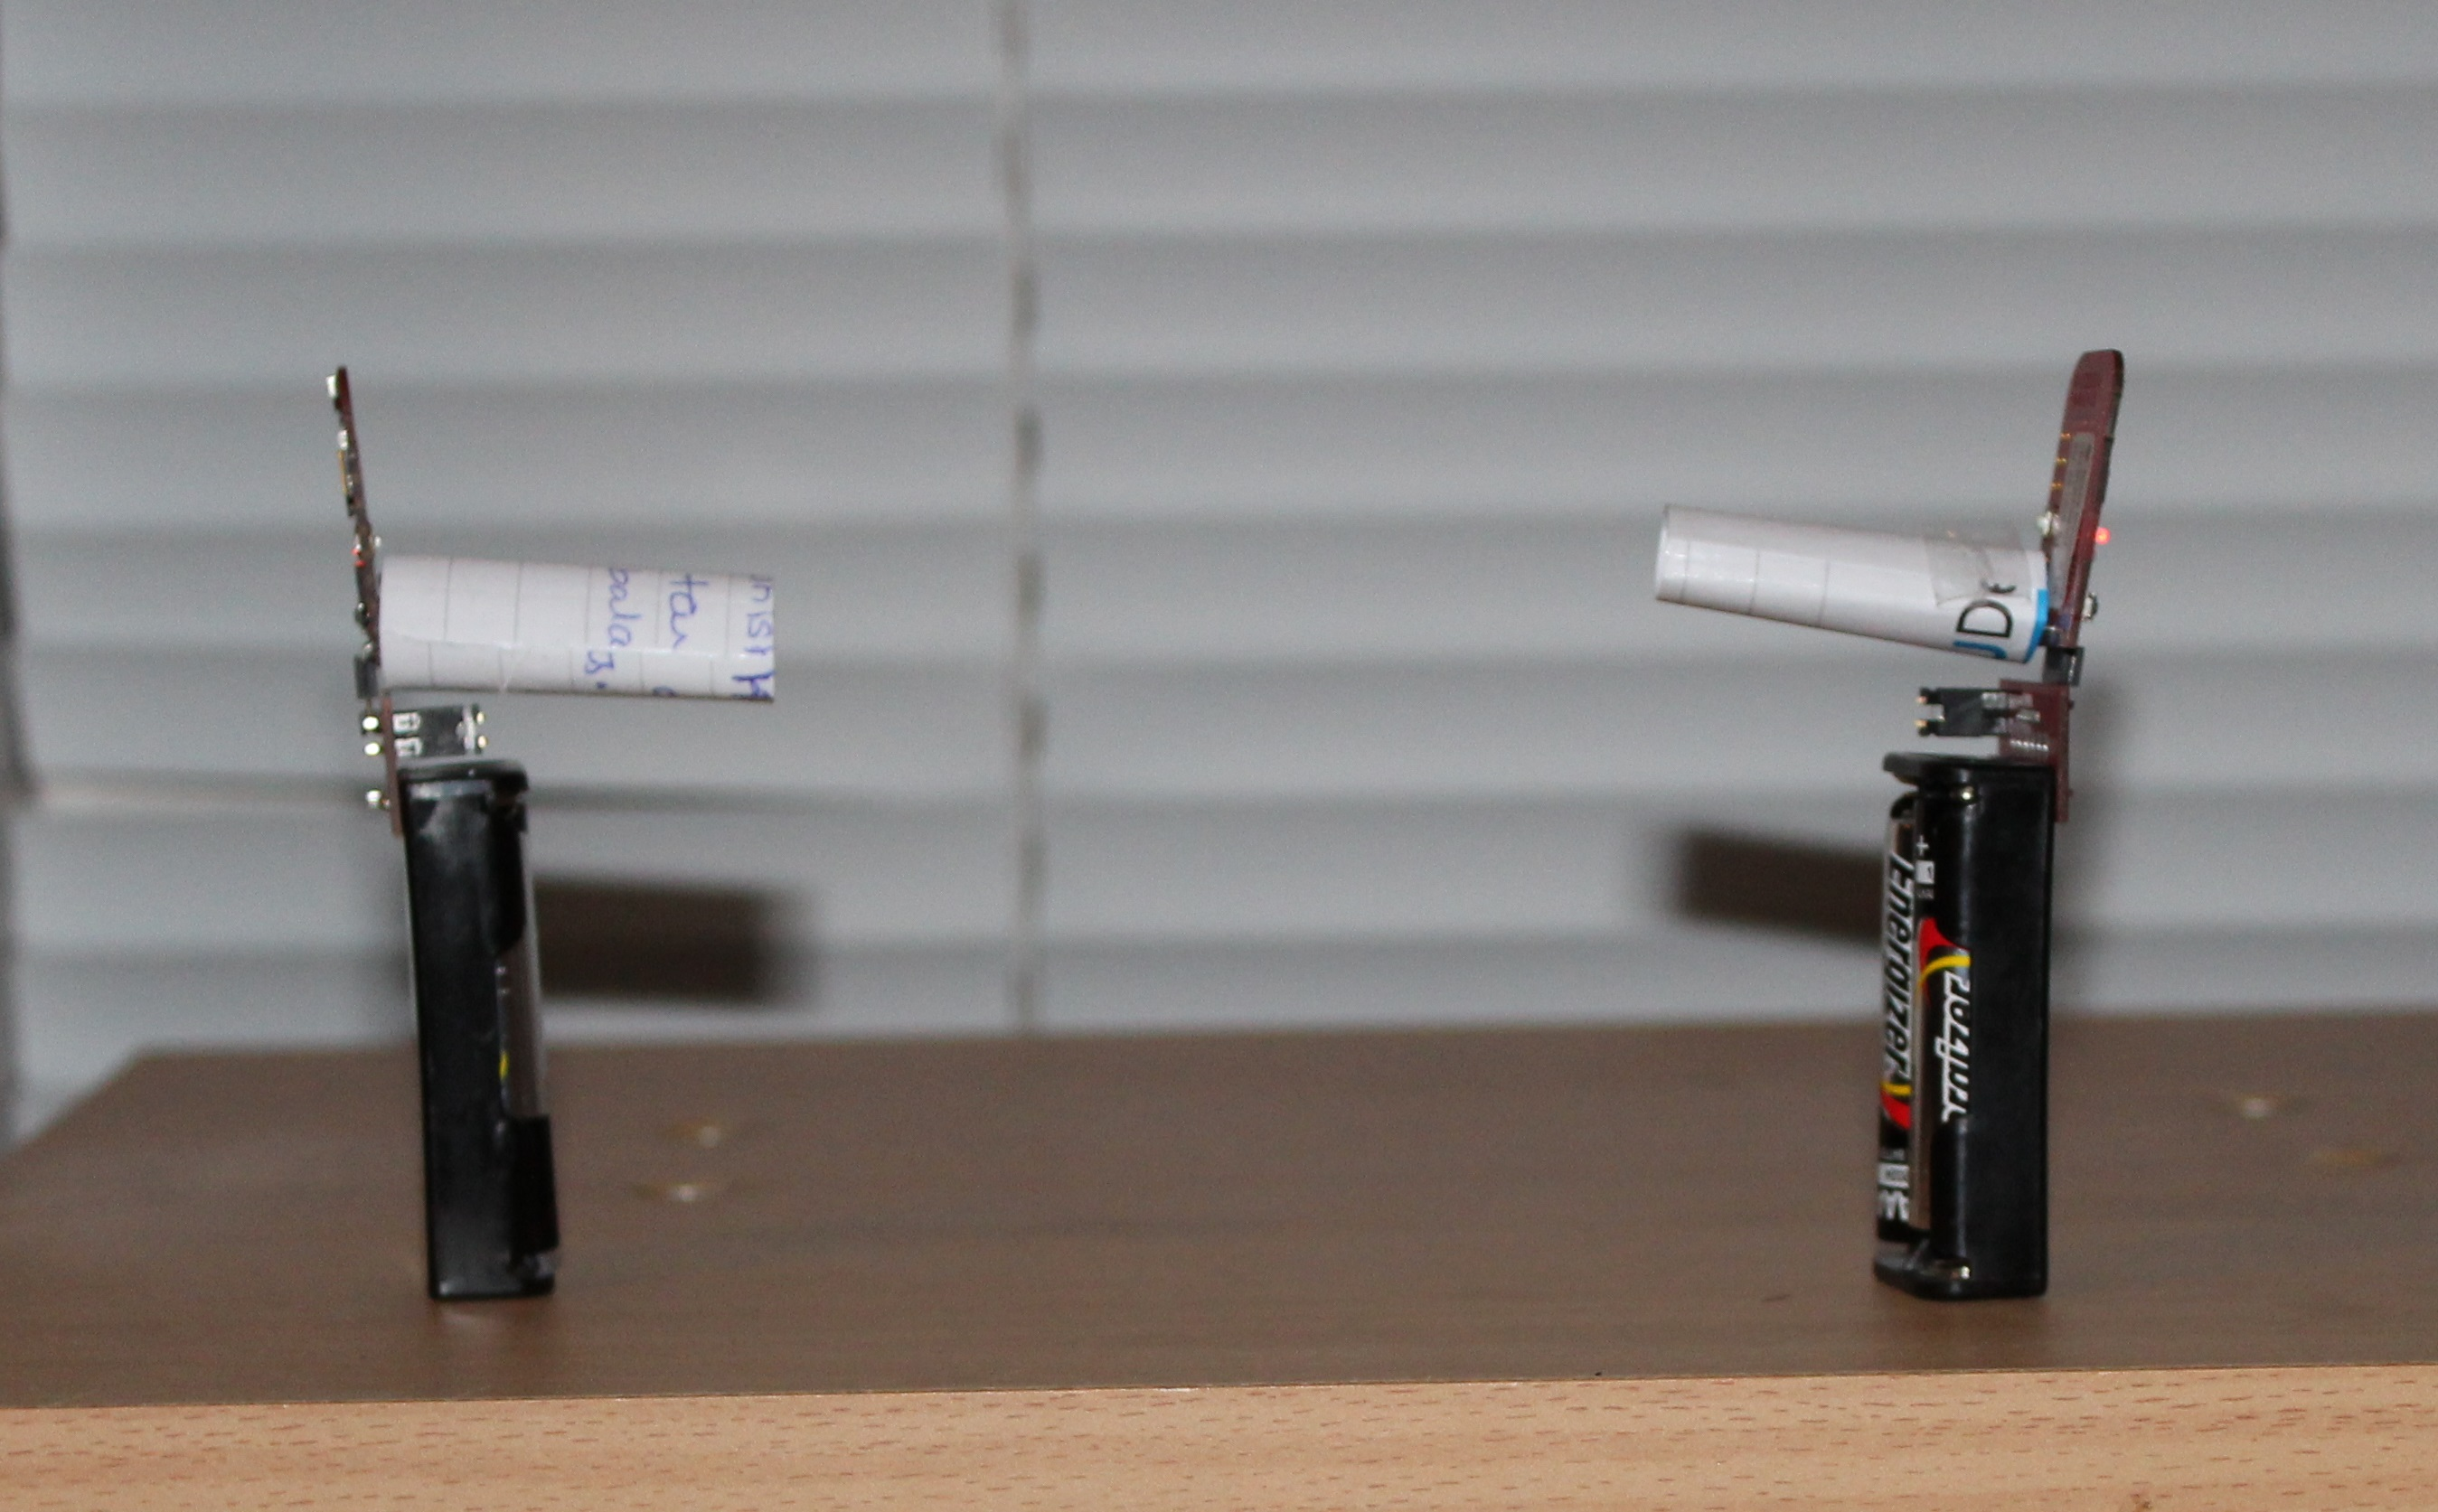
\includegraphics[scale=0.1]{./pics/timesync.jpg}
\caption{Setup to test time synchronization}
\label{fig:timeSync}
\end{figure}

\begin{figure}
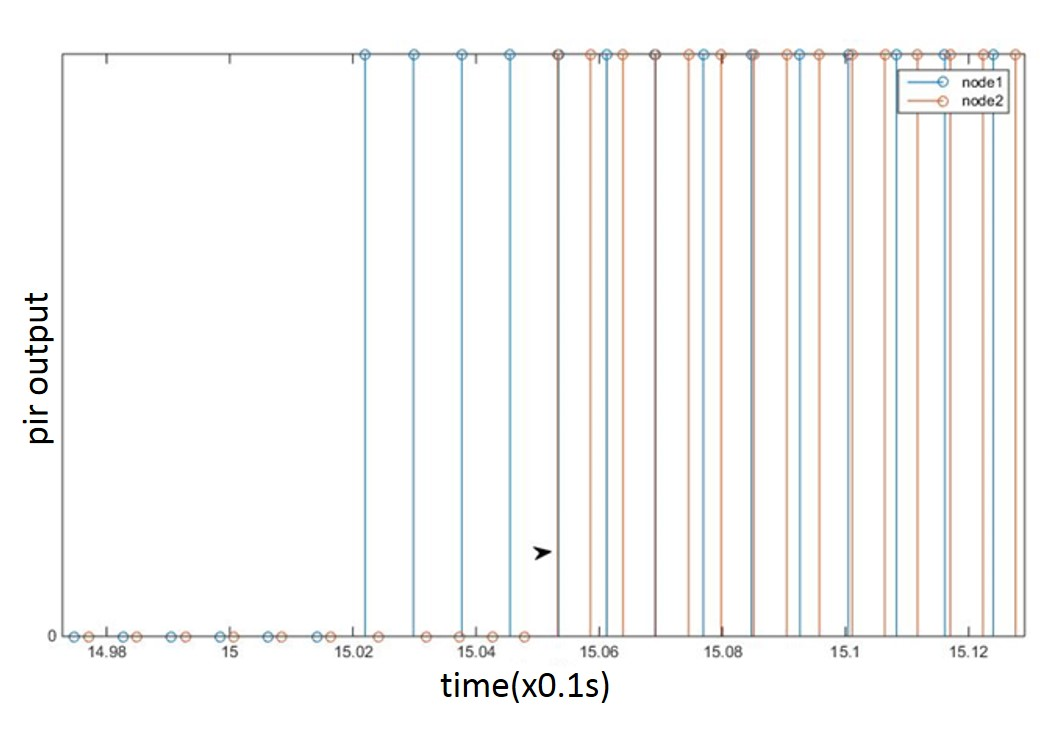
\includegraphics[scale=0.5]{./pics/timeSyncErr}
\caption{Worst case time synchronization error between two nodes}
\label{fig:timeSyncErr}
\end{figure}

To test the time synchronization we place two sensor nodes opposite to each other as shown in the Figure \ref{fig:timeSync}. We sample the sensors at 10ms. To limit the field of view of the sensors we cover the sensor with paper roll. We introduce an obstacle swiftly between the sensor for a short period. This process is repeated 10 times and the worst case time synchronization error is as shown in the Figure \ref{fig:timeSyncErr}. As can be seen in the figure the worst case time synchronization error is approximately equal to 40ms, which is acceptable for our application.

\section{Packet Structure}
In our testbed, we sample our occupancy sensors once every 100ms. Since the data is binary we combine 32 samples and transmit the packet every 3.2s. This decreases the traffic in the sensor network.
The transmitted packet is an array of unsigned integer of size one byte. Consisting of 14 bytes of payload. The payload structure is as shown in the Figure \ref{fig:packetStructure}
\begin{figure}[!ht]
 \bytefieldsetup{bitheight=3em}
\begin{bytefield}[bitwidth=2.5em]{14}
\bitheader{0-13} \\
\bitbox{1}{\tiny Mac id} & \bitbox{1}{\tiny packet number} &
\bitbox{4}{start time}
& \bitbox{4}{end time} & \bitbox{4}{data}
\end{bytefield}.
\caption{Packet Structure}
\label{fig:packetStructure}
\end{figure}

\begin{itemize}
\item Mac Id - unique identifier for each node. Mac Id is used to assign the packets received to the particular node. 
\item Packet number- Keeps track of the packets that are being transmitted from a  node. It helps to identify the lost packets as well as repeated packets. If two packets from the same node have the same packet number then they are treated as duplicate packets. If there is a packet number missing then we treat that as a lost packet.
\item Start time - 4 byte array corresponding to the time of first occupancy sensor sample in the packet.  
\item End time - 4 byte array corresponding to the time of the last occupancy sensor sample in the packet.
\item Data - 4 byte array which is combined and converted to binary form. This represents 32 samples of the occupancy sensor output. Each sample separated by an interval of 100ms. 
\end{itemize}
\section{Data Collection}
Data was collected for a span of 2 months. During the course of the evaluation, the occupants were notified of data gathering, but were never instructed to behave in any particular way or was there any constrained applied on the activity or the number of people in the room. All nodes directly communicated to a centrally located AP, which was connected to a laptop which was used to store the data. We collected a total of approximately 120hrs of data. Figure \ref{fig:dataFig} shows a part of the binary data obtained from the testbed.
\begin{figure}[!ht]
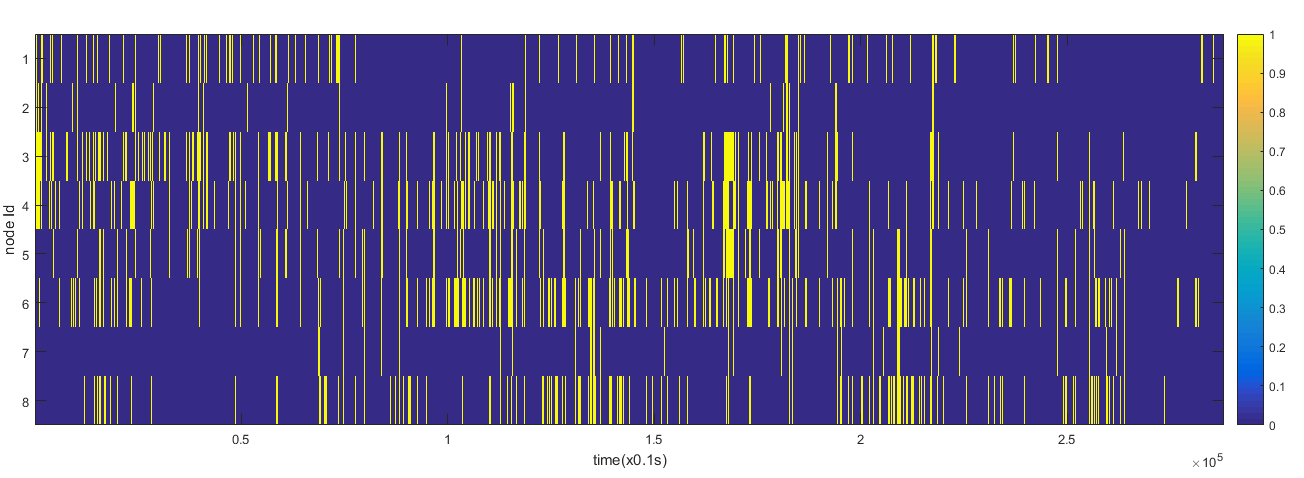
\includegraphics[width=\textwidth]{./pics/data.png}
\caption{Binary data obtained from the testbed spanning for 8hrs}
\centering
\label{fig:dataFig}
\end{figure}




\chapter{Conclusions and Future Work}
\label{chp:conclusionsandfuturework}

\section{Conclusions}
We present a new data driven method to identify the location of the sensors within a facility. We first identify a feature for the occupancy sensor data and calculate the correlation coefficient for the obtained feature data stream between the sensors. From the correlation values, we build correlation matrix ($R$)  which aids in identifying the neighboring sensor nodes. By computing the MST for $R$ we could identify at least one of the neighbors per sensor node. With the help of the coordinates of the vertices of the grid location, we model the grid as a graph and using the grid graph and the MST we reduce the problem of locating the sensors on the grid to a well-known problem of graph matching. We use the VF2 algorithm, a well known graph matching algorithm to map the sensor nodes to their locations on the grid. We validate the method developed with data from two different testbeds. We are able to identify the sensor locations with 0\% error for our experimental testbed and $4\times3$ sub-layout grid for Tokyo testbed. For the entire layout of the Tokyo testbed, we were able to identify the location of all the 43 sensors except 3.  


\section{Future Work}
The results are encouraging, going forward we would like to address the following issues in the future:

\begin{itemize}
\item Determine the effect of overlapping region on the performance of the algorithm: As could be seen while evaluating the performance of our results with the Tokyo testbed, we could notice that the length of data required to obtain accurate results varied. One of the main factors could be the extent of overlap between the sensors. In the future, we would like to investigate the effect of overlapping region on the performance of our algorithm.
\item We are only able to identify the location of the sensors up to rotational symmetry. To overcome rotational symmetry and obtain the exact location of the sensors, extra information about the space is required. For our testbed, we can make use of the location of the door and observe the sensors which are triggered last before a large period of inactivity,this basically represents the last person leaving the room. The sensors which observe the last triggers can be placed on the side of the door and thus eliminating rotational symmetry in one direction. But this method cannot be generalized to all testbed. Therefore we would like to investigate methods which will be effective to eliminate the problem caused due to rotational symmetry.
\item Apply our approach to work with other sensors: In our work, we determine the location of the sensors using the correlation matrix obtained from the occupancy sensor data.
In the future, we would like to extend our method to other sensors. The modification that would have to be done to our approach would be to identify feature for the sensor data stream for which we can compute correlation values for the sensors. If we are able to obtain a correlation matrix such that the correlation values are high for neighboring sensors and low for non neighboring sensors, we could use our method to obtain the location of the sensors.
\item We have developed this method under the assumption that the grid is a connected graph, i.e every sensor has at least one neighboring sensor. In practice, it may not be the case that the grid will always be a connected graph, therefore we would like to expand our method such that it will be able to locate the sensors even when the grid is not a connected graph.
\end{itemize}


% BIBLIOGRAPHY
%#define SORTED 1
\bibliographystyle{plainnat}
\bibliography{./bib/mycollection}




%\appendix

%\chapter{Experimental Testbed}
\label{app:A}

\begin{wrapfigure}{r}{5.5cm}
\includegraphics[width=5.5cm]{./pics/angle.png}
\label{fig:height}
\end{wrapfigure}
The coordinates of the vertices are as given in the table \ref{tab:htc34xy}. We use EKMB1101112 PIR sensors from Panasonic, with detection angle of $82^\circ$.
PIR nodes are placed on the ceiling which is at a height of 3m. From this information we can compute the radius of the field of view of the PIR sensors as follows:\\\\
$h=3m, a = 82^{\circ}$\\
$r=h\cdot tan(\frac{a}{2})$\\
$r=2.6m$\\






\begin{table}[]
\centering
\caption{Coordinates of the vertices of the sensor network}
\label{tab:htc34xy}
\begin{tabular}{|c|c|c|}
\hline
vetrex & x   & y   \\ \hline
1      & 0   & 0   \\ \hline
2      & 0   & 2.2 \\ \hline
3      & 2.5 & 0   \\ \hline
4      & 2.5 & 2.2 \\ \hline
5      & 5   & 0   \\ \hline
6      & 5   & 2.2 \\ \hline
7      & 7.5 & 0   \\ \hline
8      & 7.5 & 2.2 \\ \hline
\end{tabular}
\end{table}

\begin{table}[]
\centering
\caption{Euclidean distances between vertices}
\label{tab:dist}
\begin{tabular}{|c|c|c|c|c|c|c|c|c|}
\hline
vertices & 1    & 2    & 3    & 4    & 5    & 6    & 7    & 8    \\ \hline
1        & 0.00 & 2.00 & 2.50 & 3.20 & 5.00 & 5.39 & 7.50 & 7.76 \\ \hline
2        & 2.00 & 0.00 & 3.20 & 2.50 & 5.39 & 5.00 & 7.76 & 7.50 \\ \hline
3        & 2.50 & 3.20 & 0.00 & 2.00 & 2.50 & 3.20 & 5.00 & 5.39 \\ \hline
4        & 3.20 & 2.50 & 2.00 & 0.00 & 3.20 & 2.50 & 5.39 & 5.00 \\ \hline
5        & 5.00 & 5.39 & 2.50 & 3.20 & 0.00 & 2.00 & 2.50 & 3.20 \\ \hline
6        & 5.39 & 5.00 & 3.20 & 2.50 & 2.00 & 0.00 & 3.20 & 2.50 \\ \hline
7        & 7.50 & 7.76 & 5.00 & 5.39 & 2.50 & 3.20 & 0.00 & 2.00 \\ \hline
8        & 7.76 & 7.50 & 5.39 & 5.00 & 3.20 & 2.50 & 2.00 & 0.00 \\ \hline
\end{tabular}
\end{table}

The distances between all the sensor nodes are represented in a matrix form and is as given in the table \ref{tab:dist} . The radius of the PIR sensor is 2.6m thus any 2 sensors located less than 5.2m(2r) apart are considered neighboring sensors. The adjacecy matrix is obtained as shown in the table \ref{tab:am}

\begin{table}[]
\centering
\caption{Adjacency matrix}
\label{tab:am}
\begin{tabular}{|c|c|c|c|c|c|c|c|c|}
\hline
vertices & 1 & 2 & 3 & 4 & 5 & 6 & 7 & 8 \\ \hline
1        & 0 & 1 & 1 & 1 & 1 & 0 & 0 & 0 \\ \hline
2        & 1 & 0 & 1 & 1 & 0 & 1 & 0 & 0 \\ \hline
3        & 1 & 1 & 0 & 1 & 1 & 1 & 1 & 0 \\ \hline
4        & 1 & 1 & 1 & 0 & 1 & 1 & 0 & 1 \\ \hline
5        & 1 & 0 & 1 & 1 & 0 & 1 & 1 & 1 \\ \hline
6        & 0 & 1 & 1 & 1 & 1 & 0 & 1 & 1 \\ \hline
7        & 0 & 0 & 1 & 0 & 1 & 1 & 0 & 1 \\ \hline
8        & 0 & 0 & 0 & 1 & 1 & 1 & 1 & 0 \\ \hline
\end{tabular}
\end{table}

\chapter{Tokyo Testbed}
\label{app:B}

The coordinates of the vertices in Tokyo testbed are not explicitly specified. The information available are the room layout map as shown in figure \ref{fig:casas}, pir sensor field of view given as $1.2m \times 1.2m$ and the average distance between the sensors as 1.2m in \cite{crandall2011tracking}. Assuming that the given layout is to scale and the distance between sensors 27 and 22 as 1.2m, the coordinates of all the sensors are computed. We start by placing the origin(0,0) at vertex 30 and measure the distance of every vertex from the x and y axis which gives the coordinates of all vertices on the grid. The coordinates thus obtained are as shown in the table \ref{tab:wsuxy}. No triggers was found for sensor 38 in the dataset, hence sensor 38 is not considered.

Adjacency between two vertices is determined if the square of dimension $1.2 \times 1.2$ drawn around the vertices have any overlap. If there is any overlap then the vertices are considered neighbors.


\begin{table}[]
\centering
\caption{Coordinates obtained for the vertices}
\label{tab:wsuxy}
\begin{tabular}{|c|c|c|c|c|c|c|c|c|c|c|c|}
\hline
vertices & x    & y     & vertices & x    & y     & vertices & x     & y     & vertices & x     & y     \\ \hline
1        & 4.40 & 5.60  & 12       & 3.60 & 0.00  & 23       & 1.20  & 2.00  & 34       & -0.60 & 5.00  \\ \hline
2        & 4.40 & 4.00  & 13       & 3.60 & -1.20 & 24       & 1.20  & 0.80  & 36       & -1.40 & 4.40  \\ \hline
3        & 4.40 & 3.20  & 14       & 2.40 & 3.60  & 25       & 1.20  & 0.00  & 37       & -1.80 & 4.80  \\ \hline
4        & 4.80 & 1.20  & 15       & 2.40 & 3.20  & 26       & 1.20  & -1.20 & 39       & -1.40 & -0.20 \\ \hline
5        & 4.80 & 0.00  & 16       & 2.40 & 2.00  & 27       & 0.00  & 3.20  & 40       & -2.20 & 1.88  \\ \hline
6        & 4.80 & -1.20 & 17       & 2.40 & 0.80  & 28       & 0.00  & 2.00  & 41       & -2.20 & 0.68  \\ \hline
7        & 3.40 & 5.60  & 18       & 2.40 & 0.00  & 29       & 0.00  & 0.80  & 42       & -2.20 & -0.52 \\ \hline
8        & 3.40 & 4.40  & 19       & 1.20 & 4.80  & 30       & 0.00  & 0.00  & 43       & -3.40 & 1.88  \\ \hline
9        & 3.40 & 3.20  & 20       & 0.60 & 4.64  & 31       & 0.00  & -1.20 & 44       & -3.40 & 0.68  \\ \hline
10       & 3.90 & 2.00  & 21       & 1.20 & 3.60  & 32       & -1.20 & -0.40 & 45       & -3.40 & -0.52 \\ \hline
11       & 3.60 & 1.20  & 22       & 1.20 & 3.20  & 33       & -0.60 & 3.80  &          &       &       \\ \hline
\end{tabular}
\end{table}











\end{document}

